\begin{appendix}
\clearpage
\section{List some items}
\begin{itemize}
    \item First item
    \item Second item
    \item Another item
    \begin{itemize}
        \item Subitem
        \begin{itemize}
            \item Subsubitem
            \begin{itemize}
                \item Subsubsubitem --- Just joking, You should not use such 
                    deep nested Lists.
            \end{itemize}
        \end{itemize}
    \end{itemize}
    \item[+] Even special symbols are possible
    \item[$\sum$] Which can also be in math mode
\end{itemize}

\subsection{Enumered list}
\begin{enumerate}
    \item First item
    \item Second item
    \item Another item
    \begin{enumerate}
        \item Subitem
        \begin{enumerate}
            \item Subsubitem
            \begin{enumerate}
                \item Subsubsubitem --- Just joking, You should not use such 
                    deep nested Lists.

            \end{enumerate}
        \end{enumerate}
    \end{enumerate}
\end{enumerate}

% BLDC

\includepdf[
    pages=1, 
    offset=0cm -2.5cm, 
    frame=false, 
    pagecommand={
        \textcolor{white}{\section{Anhang: Dokumentation BLDC Motor Treiber}}
        \label{app:bldc}
        \thispagestyle{empty}}
    ]{cd/BLDC_StandaloneDoc.pdf}

\includepdf[
    pages=2-, 
    offset=0cm -2.5cm, 
    frame=false, 
    pagecommand={
        \thispagestyle{empty}}
    ]{cd/BLDC_StandaloneDoc.pdf}
% Stepper

\includepdf[
    pages=1, 
    offset=0cm -2.5cm, 
    frame=false, 
    pagecommand={
        \textcolor{white}{\section{Anhang: Dokumentation Schrittmotor Treiber}}
        \label{app:stepper}
        \thispagestyle{empty}}
    ]{cd/Stepper_StandaloneDoc.pdf}

\includepdf[
    pages=2-, 
    offset=0cm -2.5cm, 
    frame=false, 
    pagecommand={
        \thispagestyle{empty}}
    ]{cd/Stepper_StandaloneDoc.pdf}
% DC

\includepdf[
    pages=1, 
    offset=0cm -2.5cm, 
    frame=false, 
    pagecommand={
        \textcolor{white}{\section{Anhang: Dokumentation DC Motor Treiber}}
        \label{app:dc}
        \thispagestyle{empty}}
    ]{cd/DC_StandaloneDoc.pdf}

\includepdf[
    pages=2-, 
    offset=0cm -2.5cm, 
    frame=false, 
    pagecommand={
        \thispagestyle{empty}}
    ]{cd/DC_StandaloneDoc.pdf}
% Aufgabenstellung
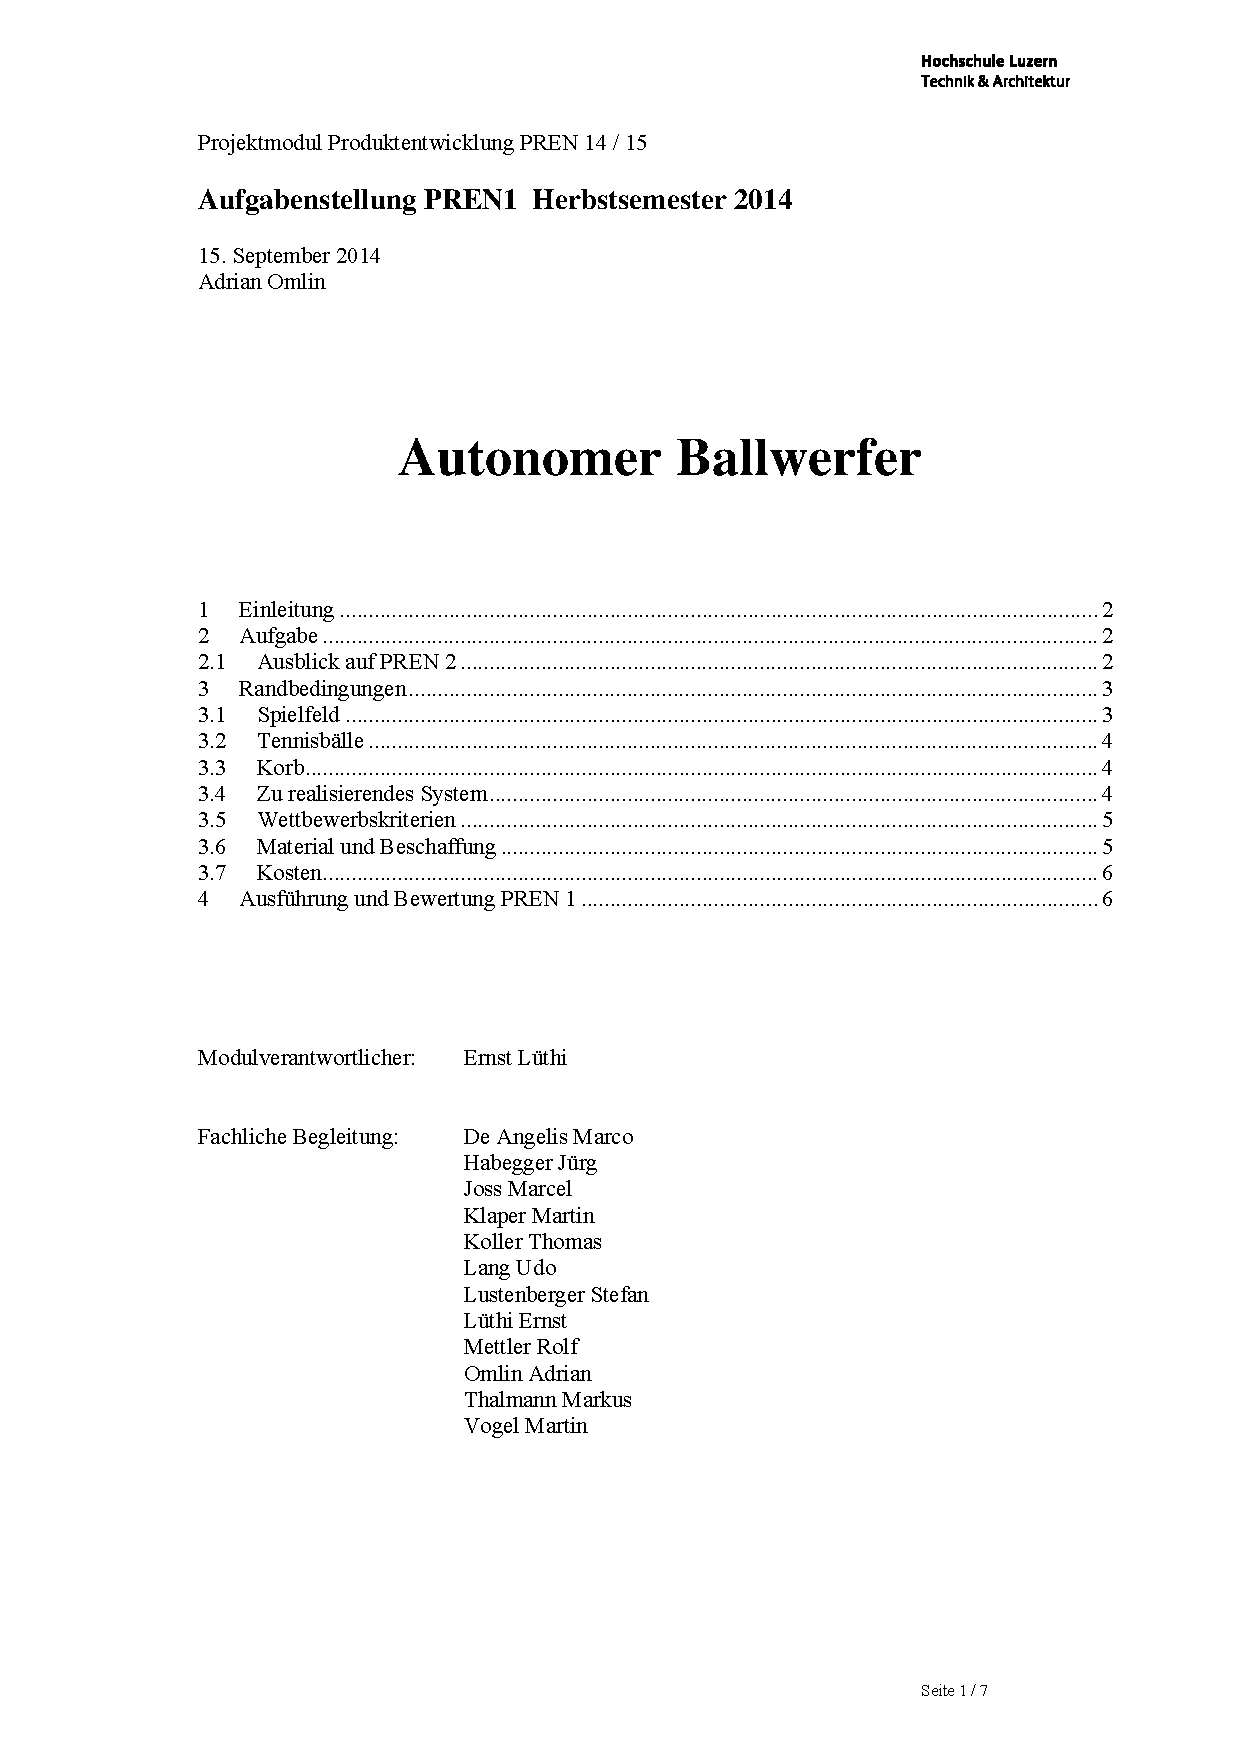
\includepdf[
    pages=1, 
    offset=0cm -2.5cm, 
    frame=false, 
    pagecommand={
        \textcolor{white}{\section{Anhang: Aufgabenstellung}}
        \label{app:aufgabe}
        \thispagestyle{empty}}
    ]{cd/Aufgabenstellung_PREN1_H14.pdf}
\includepdf[
    pages=2-, 
    offset=0cm -2.5cm, 
    frame=false, 
    pagecommand={
        \thispagestyle{empty}}
    ]{cd/Aufgabenstellung_PREN1_H14.pdf}
\end{appendix}
